\documentclass[a4paper, 11pt]{article}

\usepackage{amsmath}
\usepackage{amssymb}
\usepackage{amsthm}
\usepackage{url}
\usepackage{graphicx}
\usepackage{caption}
\usepackage{subcaption}
\usepackage{hyperref}


\begin{document}

\title{Contagion of an exogenous failure in a bank network}
\date{\today}
\author{Marco Tinacci}
\maketitle

All the material of this work, including the up-to-date version of this document, can be found in the public repository \url{https://github.com/marcotinacci/interbank-lending-systemic-risk}.

\section{Introduction} % (fold)
\label{sec:introduction}
We take under consideration large banking systems. In \cite{KrauseGiansante} many real examples of systems are considered and they propose a taxonomy in which tiering and size are the two orthogonal dimensions. We can model this kind of system as a network where connections represent interbank loans. We have a high level of tiering when a few banks dominate the majority of connections, like the UK and Italian market.

We want to analyze what happens when the an exogenous shock make the biggest bank fail generating a chain of losses to other connected banks. To do that we implement a generator of realistic banking systems and the propagation mechanism and we run some simulation to check how the failure spreads if we change some system parameters. We will describe decisions that has not been specified in \cite{KrauseGiansante} and we will focus on how the contagion mechanism changes when banks adopt heterogenous model of loans (to customers or to other banks) and when they adopt an homogenous model, in our case, a model focused on loans to customers.

% section introduction (end)

\section{Model} % (fold)
\label{sec:model}

\paragraph{Bank network} % definizione grafo orientato pesato
To build the bank network we take the model adopted in \cite{KrauseGiansante}. The single bank is represented by a node of the network and contains some information about the internal balance. Formally we define a node $\mathcal{B}$ as follows
$$ B = \langle A,\rho,\beta,\gamma,\alpha \rangle $$
such that $A \in \mathbb{R}$, $\rho,\beta,\gamma,\alpha \in [0,1]$, $\rho + \beta \leq 1$ and $\gamma + \alpha \leq 1$. $A$ is the asset of $B$, $\rho \cdot A$ are cash reserves, $\beta \cdot A$ are loans to customers and $(1-\rho-\beta) \cdot A$ are loans to other banks. Other fractions are liabilities: $\gamma \cdot A$ are deposits by customers, $\alpha \cdot A$ is the equity and $(1-\gamma-\alpha) \cdot A$ are loans received from other banks. We will consider two main failure condition of a bank: $\rho = 0$ and $\alpha = 0$.

To denote different nodes we use a subscript notation $B_i$ and the same for its internal data $A_i,\rho_i,\beta_i,\gamma_i,\alpha_i$. We denote with $\mathcal{B}$ the set of all the banks taken into account in our system.
Interbank loans are represented by the relation $L \subseteq \mathcal{B} \times \mathbb{R^+} \times \mathcal{B}$ and we say that $(B_1,l,B_2) \in L$ when bank $B_1$ lend $l$ to $B_2$, we can also write $B_1 \xrightarrow{l} B_2$.
Now we can define the banking system network as a directed weighted graph $\mathcal{G} = \langle \mathcal{B}, L \rangle$ where $\mathcal{B}$ is the set of bank nodes and $L$ is the relation that contains all the oriented and weighted edges between nodes.

\paragraph{Asset and degree distribution} % asset e gradi come power law
Since we want a random network as close to a realistic scenario as possible, we need to generate bank assets as a power law distribution, to be precise we use the following probability density function
$$ f_{pdf}(x;a) = C x^{-a} $$
where $C \in \mathbb{R}$ is a scaling factor computed such that $f_{pdf}$ is a proper probability density function in the desired range. $a$ is a simulation parameter and is decided depending on the kind of network we want to generate, $C$ will depend on $a$. Internal information $\rho,\beta,\gamma,\alpha$ are chosen uniformly at random in given ranges. Let us denote with $\mathcal{B}^a$ the set of bank nodes generated at random as just described. Also the degree distribution must follow a power law distribution and, to be realistic, we need it to be strongly correlated to the assets distribution. To obtain this we use the algorithm to generate the Chung Lu model \cite{ChungLu} that returns a random (selfloop-free) graph with given expected degrees. Every edge between $B_1$ and $B_2$ is generated with probability 
$$ p_{B_1B_2} = \frac{w_{B_1}w_{B_2}}{\sum_B w_B} $$
where $B_1,B_2 \in \mathcal{B}$ and $w_{B_1}, w_{B_2}$ are respectively their expected degree. We use normalized assets of nodes as expected degrees, in this way we obtain a degree distribution strongly correlated to the assets distribution (Figure~\ref{fig:corr}).

\begin{figure}[htbp]
    \centering
    \begin{subfigure}[b]{0.6\textwidth}
		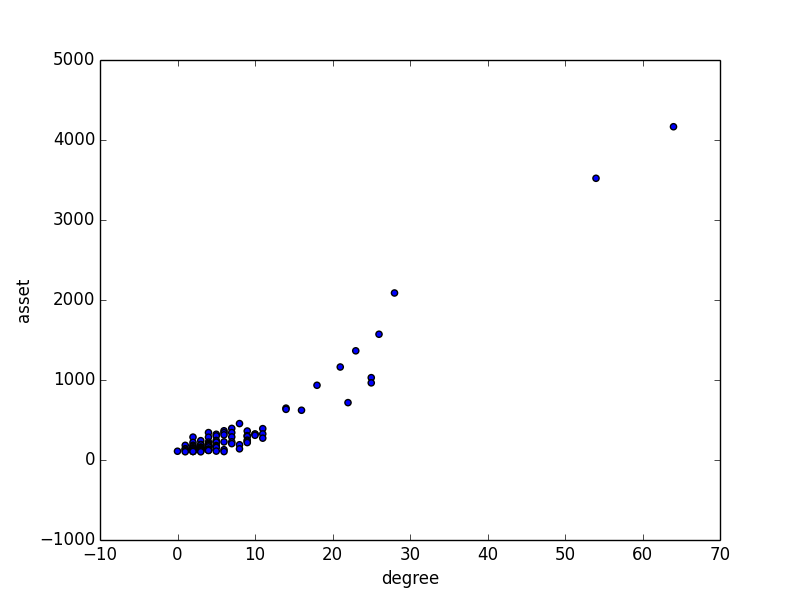
\includegraphics[width=\textwidth]{images/scatter2.png}
        \caption{$a = 2, \rho=0.96$}
	\end{subfigure}
    \begin{subfigure}[b]{0.6\textwidth}
		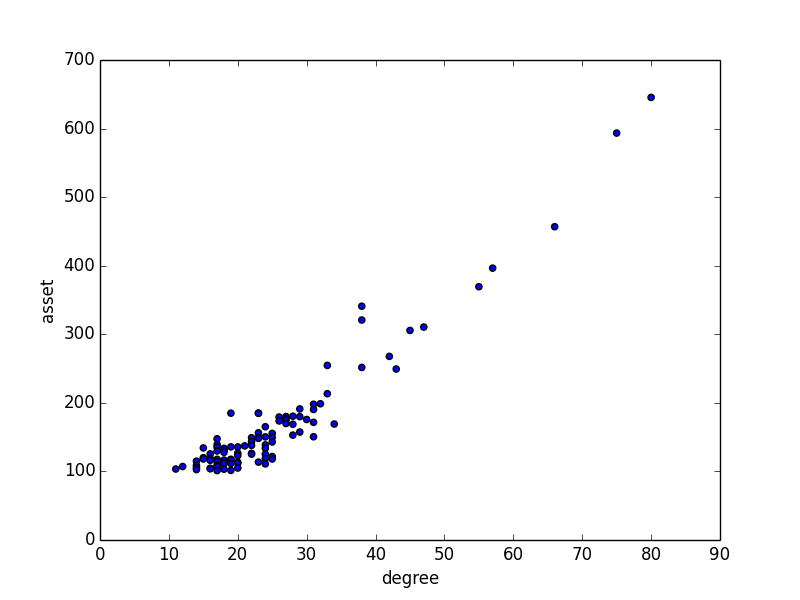
\includegraphics[width=\textwidth]{images/scatter3.png}
        \caption{$a = 3, \rho=0.96$}
	\end{subfigure}
    \begin{subfigure}[b]{0.6\textwidth}
		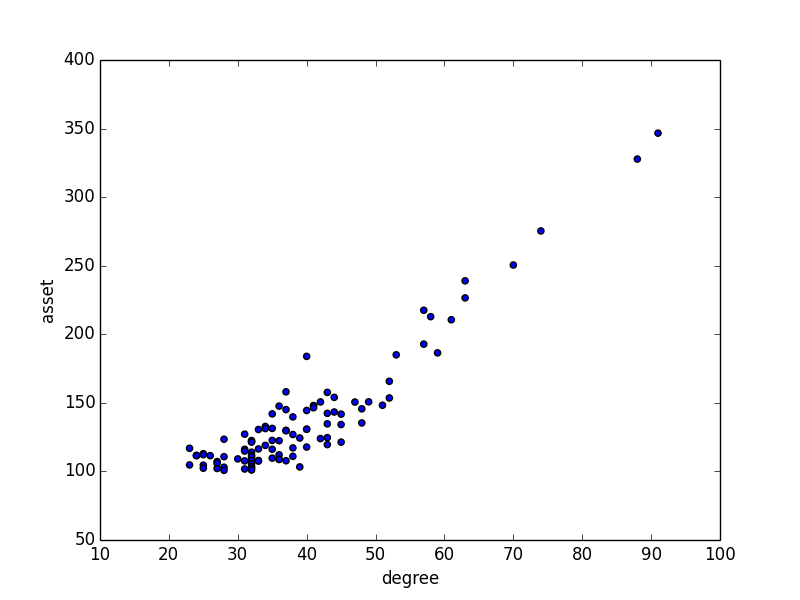
\includegraphics[width=\textwidth]{images/scatter4.png}
        \caption{$a = 4, \rho = 0.93$}
	\end{subfigure}
	\caption{Scatter plots between degrees and assets generated trough power laws with different exponent $a$. The minimum correlation $\rho$ is $0.93$}\label{fig:corr}
\end{figure}

Since a loan is naturally modeled as an \emph{oriented} edge, we need to modify the graph structure in order to obtain such feature, preserving the described properties. We use the following procedure: every undirected edge $(B_i, B_j)$ is replaced by a directed one, with equal probability by $(B_i,B_j)$ or $(B_j,B_i)$. This trivially guarantees that the degree (input and output) of each node in the directed graph is still following a power law distribution.

Finally we need to transform the just described directed graph to a \emph{weighted} directed graph whose weights are interbank loans' amounts. If $(B_i,B_j)$ is an edge of the directed graph then $(B_i,l,B_j)$, $B_i$ lend $l$ to $B_j$, is a weighted edge of the weighted directed graph such that 
$$l = \frac{A_j(1-\gamma_j-\alpha_j) \cdot A_i(1-\rho_i-\beta_i)}{\sum_{k \in cred(i)} A_k(1-\gamma_k-\alpha_k)}$$
where $cred(i)$ is the index set of all the creditors of bank $B_i$. Using the previous formula is easy to compute the weighted adjacency matrix. To maintain consistency with every bank balance an asset update is necessary to move the lent money from a bank to another, this however is a minor adjustment that preserves the power law distribution of assets and the correlation with the degree distribution.

\paragraph{Contagion} % meccanismi di contagio
The event we are going to simulate is the contagion of a failure after the bank with the highest asset $B_0$ fails by an exogenous event. Then $B_0$ is forced to repay its debts and, to do so, it also has to call back its loans to other banks. Calling loans in and repaying debts with respect to other banks are two mechanisms that can propagate the failure to other banks and they are called respectively \emph{failure mechanism} and \emph{default mechanism}.

In the failure mechanism every loan to another bank, say $B_c$, is called in and if the creditor bank has not enough cash to restore the debt then it goes bankrupt in turn and the initially failing bank needs to wait for the entire failing procedure of $B_c$ to recover its money. This mechanism can lead to a chain of failures and, in some cases, also in a cyclic chain. When the latter happens it means that a failing bank is calling in a loan from another failing bank, in this case we assume that this bank lose the entire loan. Another likely case is the bankrupt by combined call in of loans: this happens when $B_c$ would be able to repay debts to more than one bank individually, but if more failure happens $B_c$ does not have enough cash to repay the sum of recalled loans. Since the purpose of this procedure is transforming the whole bank asset into cash (basically $\rho = 1$) we also need to call loans to customers back, but only a part of this loans can be recovered, in our case we assume a recovery rate $k$ that is the same for every bank.

After a failing bank terminate to call in its credits it must start to repay its debts. Deposits to customers are the first to be restored, then, if some cash remains, borrowing with respect to other banks must be restored. If the failing bank is able to restore every debt to other banks then the failure cannot propagate to them. Otherwise the bank equally split its remaining cash among all the debtor banks (except for smaller debts, those below the split fraction, that are paid individually) and the difference between the actual debt and the restored part results as a loss for the debtor. This loss is recorded as a decrement of the equity in the liabilities and when equity goes to zero ($\alpha = 0$) the bank goes bankrupt and so the failure propagate. Again, it may happen that a bank would be able to sustain individual losses deriving from a partially repaid debt but it actually goes bankrupt for their summed effect.

The exogenous failure is triggered by setting the biggest bank's equity to zero, this will force it to go bankrupt and to start the contagion. In Figures~\ref{fig:network2}, \ref{fig:network3} and \ref{fig:network4} we show some examples of randomly generated network, before and after the trigger of the exogenous failure, respectively with $a=2$, $a=3$ and $a=4$. Green nodes are active banks, yellow nodes are banks failed by failure mechanism, red nodes are banks failed by default mechanism and the blue node is the trigger.

\begin{figure}[htbp]
    \centering
    \begin{subfigure}[b]{0.9\textwidth}
		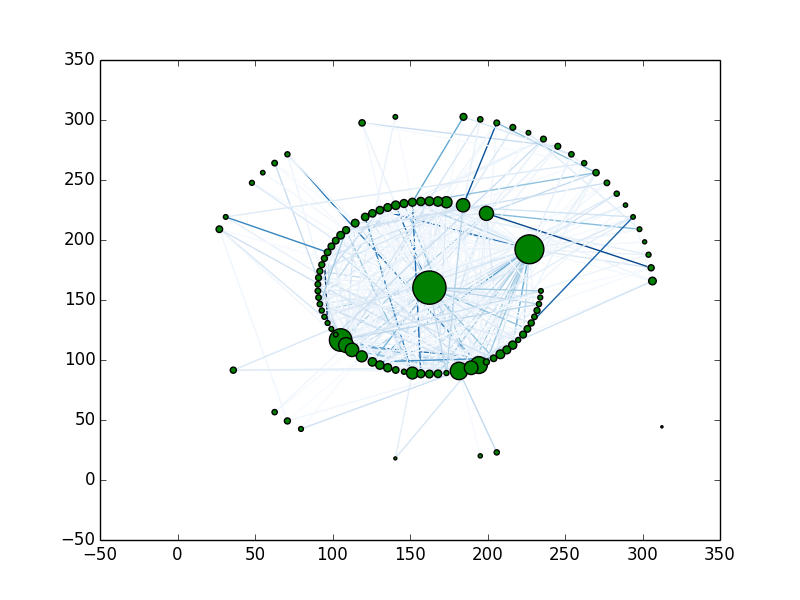
\includegraphics[width=\textwidth]{images/network2.png}
	\end{subfigure}
    \begin{subfigure}[b]{0.9\textwidth}
		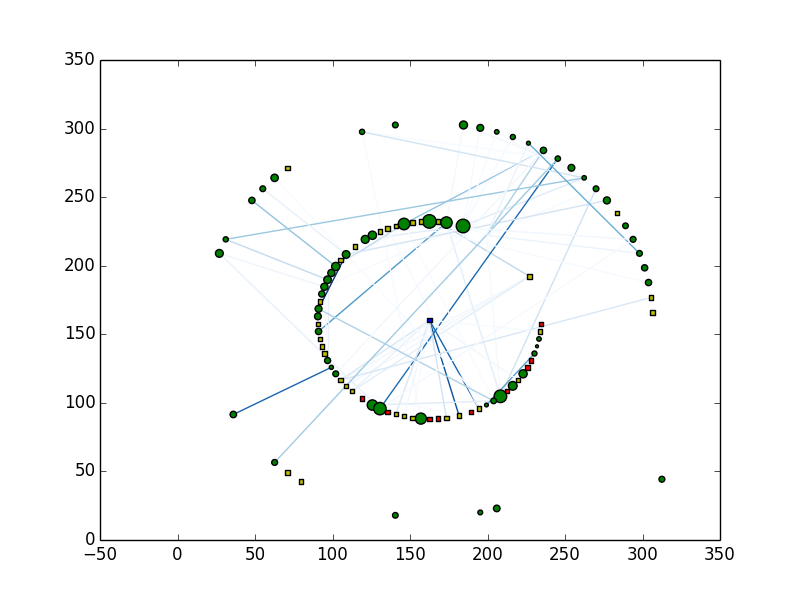
\includegraphics[width=\textwidth]{images/contagion2.png}
	\end{subfigure}
	\caption{Graphical representation of a network generated with $N = 100$ and power law exponent $a = 2$, before and after the trigger of the exogenous failure.}\label{fig:network2}
\end{figure}

\begin{figure}[htbp]
    \centering
    \begin{subfigure}[b]{0.9\textwidth}
		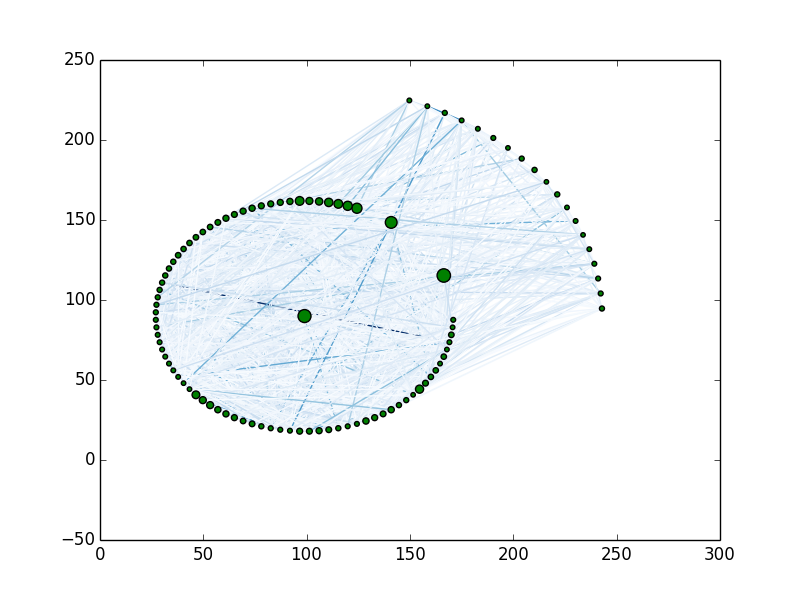
\includegraphics[width=\textwidth]{images/network3.png}
	\end{subfigure}
    \begin{subfigure}[b]{0.9\textwidth}
		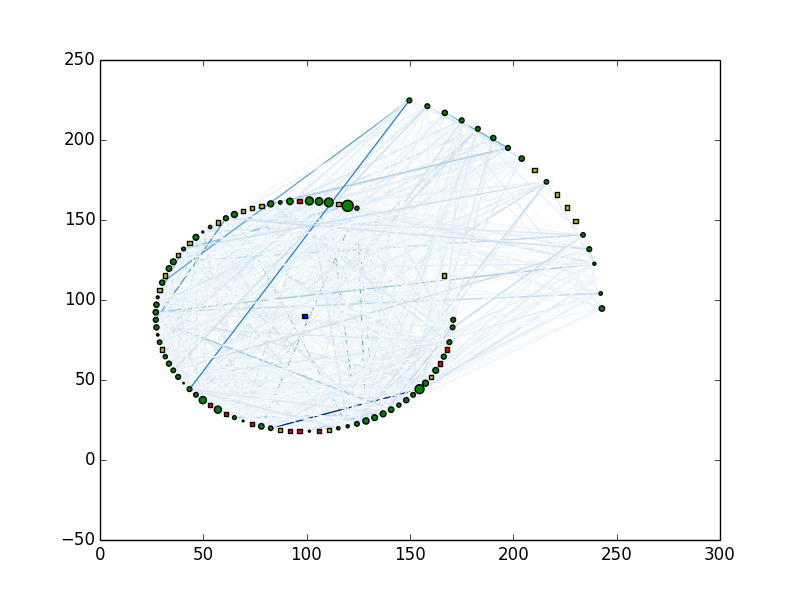
\includegraphics[width=\textwidth]{images/contagion3.png}
	\end{subfigure}
	\caption{Graphical representation of a network generated with $N = 100$ and power law exponent $a = 3$, before and after the trigger of the exogenous failure.}\label{fig:network3}
\end{figure}

\begin{figure}[htbp]
    \centering
    \begin{subfigure}[b]{0.9\textwidth}
		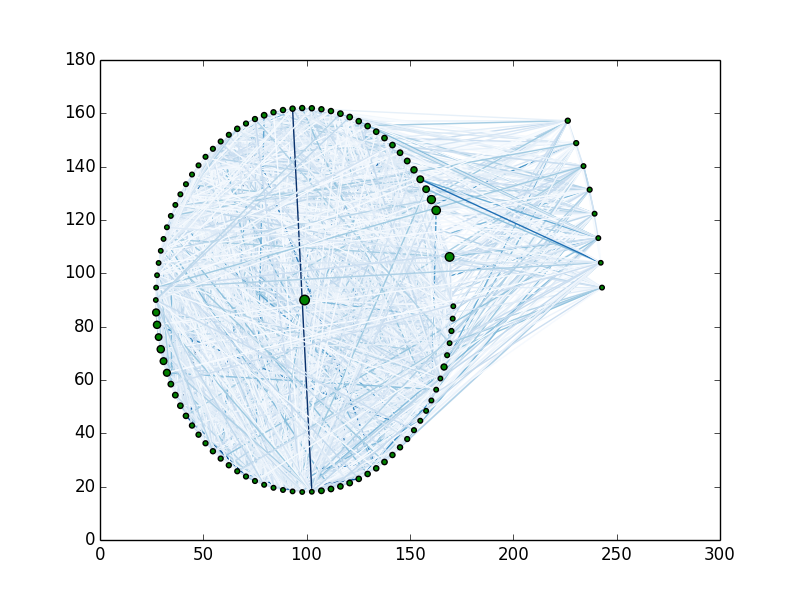
\includegraphics[width=\textwidth]{images/network4.png}
	\end{subfigure}
    \begin{subfigure}[b]{0.9\textwidth}
		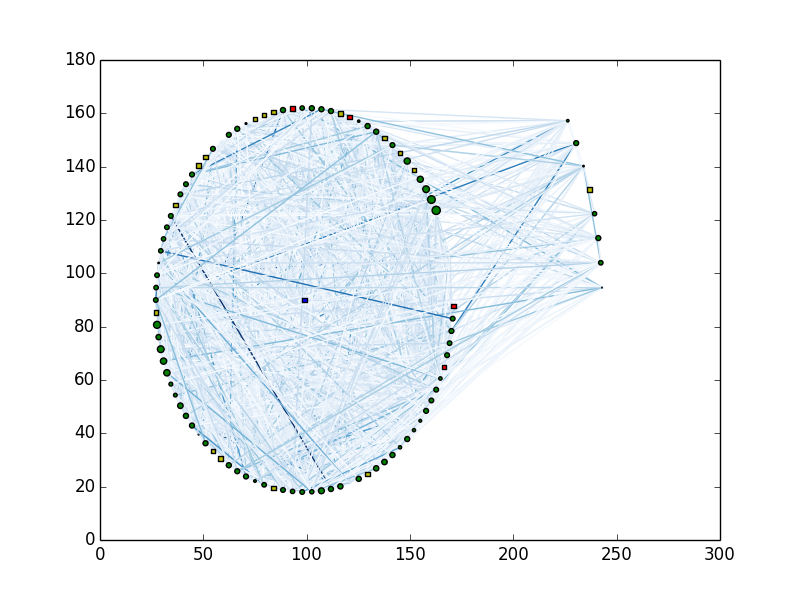
\includegraphics[width=\textwidth]{images/contagion4.png}
	\end{subfigure}
	\caption{Graphical representation of a network generated with $N = 100$ and power law exponent $a = 4$, before and after the trigger of the exogenous failure.}\label{fig:network4}
\end{figure}
 
\paragraph{Analysis}

We want to analyze how different kind of networks react to the exogenous failure of the biggest bank of the system. To do that we consider the \emph{fraction failing} index that is trivially the number of banks failed during the chain reaction divided by the initial number of banks. More specifically we want to analyze how this index changes in bank networks where nodes have higher (or lower) fractions of loans to customers or to other banks, tuning the range in which $\beta$ is drawn. We expect to see that the higher is $\beta$ the lower is the amount of infected nodes.

% section model (end)

\section{Experiments} % (fold)
\label{sec:experiments}

We consider the following set up: bank assets $A_i \in [100;10^{10}]$ are drawn from a power law distribution with exponent $a \in \{2,3,4\}$ and recovery rate $r = 0.5$ for every bank. Bank specific fractions are drawn from uniform distribution over the following ranges: $\rho_i \in [0;0.25]$, $\beta_i \in [0;1-\rho_i]$, $\alpha_i \in [0;0.25]$ and $\gamma_i \in [0;1-\alpha_i]$. We adopt the following generalized notion of range for the customer loans fraction 
$$\beta_i^k \in \left[ k \cdot s\ ; 1-\rho_i \right]$$
for $k \in [0..niter-1]$ and the step size $s = (1-\rho_i) / niter$. $niter$ is an arbitrary number of iterations, the higher it is the finer is the analysis. Note that for $k = 0$ it boils down to the range defined initially $\beta_i^0 \equiv \beta_i$. Using this kind of variation we can observe how the fraction failing changes in a bank system where loans to customers are more or less common than interbank loans.

From simulations we obtain experimental results shown in Figures~\ref{fig:exp1}, \ref{fig:exp2} and \ref{fig:exp3}. We considered respectively network of dimension $50$, $100$ and $200$ and the plots represent how the fraction failing decrease as $k$ grows, in an average of $20$ simulations for each step. We can see that the fraction failing is always decreasing if we increase the probability of the banking system to put more effort into loans to customers instead of other banks. This is expected since bank connections will not be strong enough to reach the failure conditions when $k$ is high. Another observation to be made is that fraction failing decrease is slower when $a$ is low, moreover the fraction failing seems to be lower for initial values of $k$ but at some point the trend is always inverted. From this we can infer that a core-periphery structure is safer when loaning attitudes are heterogeneous, but it is unsafe when the general approach is based on loans to customers that will generate large losses due to the recovery rate. We can also say that a core-periphery model is harder to make safe if compared to a more homogeneous one. All these observations hold for every dimension of network analyzed in our experiments, in fact dynamics highlighted by the experiments remain evident. When we increase $N$ the only notable difference is a transversal decrease of the fraction failing, from this we can say that larger systems are more resistant to failure contagion.

\begin{figure}[htbp]
    \centering
	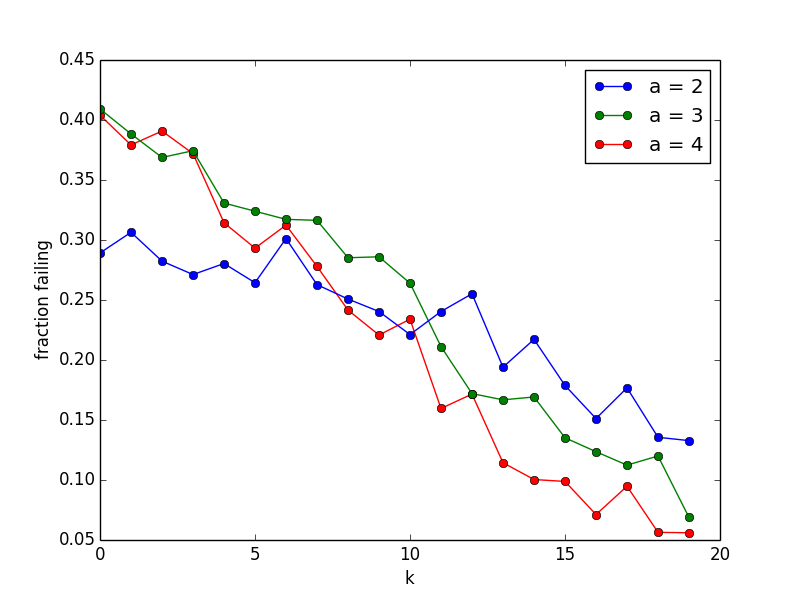
\includegraphics[width=.8\textwidth]{images/ff50.png}
	\caption{Plots of failing fraction when iterator $k$ changes, in a bank network of size $N=50$}\label{fig:exp1}
\end{figure}
\begin{figure}[htbp]
    \centering
	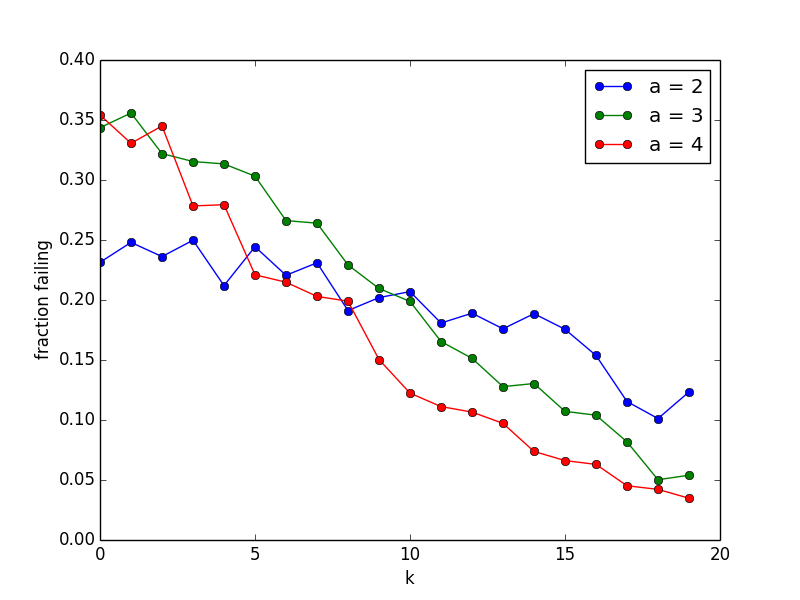
\includegraphics[width=.8\textwidth]{images/ff100.png}
	\caption{Plots of failing fraction when iterator $k$ changes, in a bank network of size $N=100$}\label{fig:exp2}
\end{figure}
\begin{figure}[htbp]
    \centering
	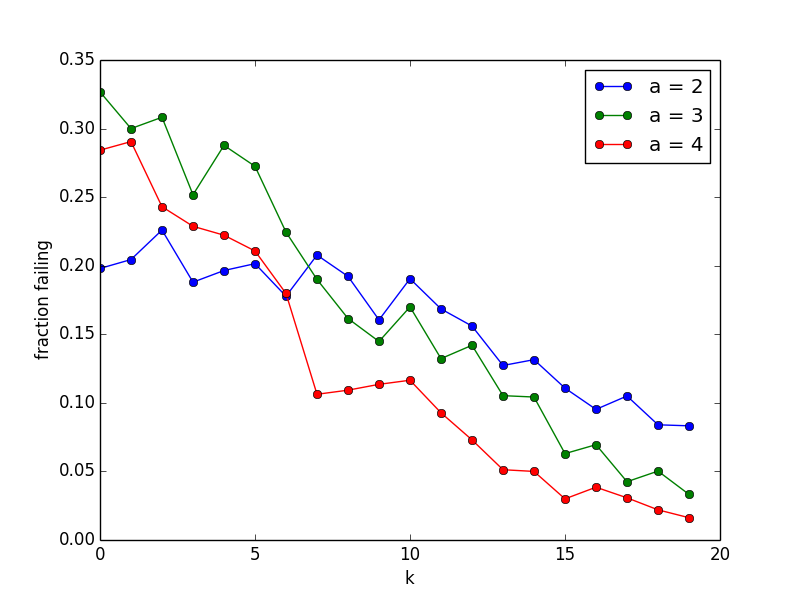
\includegraphics[width=.8\textwidth]{images/ff200.png}
	\caption{Plots of failing fraction when iterator $k$ changes, in a bank network of size $N=200$}\label{fig:exp3}
\end{figure}

% section experiments (end)

\section{Implementation} % (fold)
\label{sec:implementation}

The source code used for running simulations is completely available on \url{https://github.com/marcotinacci/interbank-lending-systemic-risk}. The code is completely written in python $2.7$, using the \texttt{Spyder} IDE for Mac. The mainly used package is NetworkX~\cite{networkx}, PyGraphviz~\cite{pygraphviz} has also been used for some graphical plot.

\texttt{Network.py} is the module dedicated to the construction of the network. \texttt{Graph} and \texttt{DiGraph}, respectively undirected and directed graph, are the main data structures employed in this code and they are provided by \texttt{networkx}. Method \texttt{initGraph(N,a)} returns an undirected graph whose nodes' information are generated randomly as described in Section~\ref{sec:experiments}, its parameters are the network dimension $N$ and the power law exponent $a$. \texttt{initGraphMod(N,a,k,niter)} is the generalized version of the previous method in which we allow the proposed range refinement. These two functions rely on the \texttt{expected\_degree\_graph(exp\_degree,selfloops} method provided by \texttt{networkx} that implements the Chung Lu model mentioned in Section~\ref{sec:model}. Method \texttt{Graph2DiGraph(g)} is used to convert the undirected graph to a directed one, then, with \texttt{WeightedEdges(g)} it is also possible to compute the amount of every interbank loan and to assign it to the respective edge as its weight. \texttt{UpdatedAssets(g)} is used to implement the initial adjustment of assets due to generated interbank loans. Used in sequence, these four methods allow the generation of the desired network.

Module \texttt{Contagion.py} is dedicated to triggering and spreading the failure reaction. \texttt{contagion(init,dg)} is the initial method that exogenously set the equity of the $init$ node to zero and start the failing procedure, $dg$ is the directed graph representing the bank network. \texttt{windup(b,dg)} is the call in procedure applied to node $b$, firstly it recovers loans from customers applying the recovery rate, then it calls interbank loans in and apply eventual losses. If the conditions are met it also triggers the failure procedure to other nodes. \texttt{repay(b,dg)} is the dual function that handle the second phase in which debts of bank $b$ are restored. Again, if the condition for the failure of a creditor are met according to the default mechanism, then the method can call the failure procedure on it. \texttt{failure(b,dg)} gather the last two methods to provide a standard failure procedure on node $b$.

We have then other secondary modules: \texttt{Plot.py} gather customized plot functions, \texttt{Measures.py} contains some measure of interest, \texttt{Statistics.py} contains the implementation of a power law distribution as a customization of the continuous random variable from package \texttt{scipy.stats}, \texttt{Test.py} contains checks and finally \texttt{main.py} and \texttt{Experiments.py} are the scripts used to glue everything together and to obtain final results.

% section implementation (end)

\bibliographystyle{plain}
\bibliography{biblio}

\end{document}
